\chapter{Testování softwaru}
Na začátek je potřeba vysvětlit některé pojmy z~oblasti testování. Budeme vycházet hlavně z~\citep{RizeniKvalitySW}, \citep{Patton} a~\citep{Herout}.

	\section{Požadavky}
	Požadavky zachycují přání zákazníka na funkcionalitu softwaru. Dělí se na dvě skupiny:
		\begin{itemize}
			\item Funkční -- popisují funkčnost služby vykonávané systémem, tedy co má vykonávat. Patří sem např.:
				\begin{itemize}
					\item Uživatel bude moci vytvořit záznam pro nového zákazníka.
					\item Systém automaticky odhlásí uživatele po 3 minutách nečinnosti.
				\end{itemize}
			\item Mimofunkční -- popisují určité vlastnosti systému, či omezující podmínky. V~podstatě říkají, jaký by systém měl být. Sem patří např.:
				\begin{itemize}
					\item Modul "Správa klientů" bude dostupný pouze uživatelům s~rolí správce.
					\item Systém bude použitelný při zátěži 1000 uživatelů.
				\end{itemize}
		\end{itemize}
	
	Je vhodné, aby se testeři zabývali i~požadavky, neboť mohou již v~rané fázi vývoje zachytit ty chybně formulované (nekonzistentní, neproveditelné, nekompletní, netestovatelné, nejednoznačné, více požadavků zapsaných jako jeden apod.).
	
	\section{Specifikace požadavků na software}
	Funkční i~mimofunkční požadavky zákazníka, jejich analýza a~dokumentace a~všeobecný popis systému se zapisuje do dokumentu nazvaného specifikace požadavků na software. Na základě tohoto dokumentu probíhají následující fáze vývoje, proto je jeho správnost velmi podstatná.
	
	K~tomuto dokumentu se poté vztahuje i~testování, konkrétně funkční testování, které kontroluje, zda software vyhovuje a~splňuje požadavky zákazníka.
	
	\section{Kvalita softwaru}
	Kvalita softwaru je velmi obtížně definovatelný pojem. Pro její definici vzniklo několik norem. Ty jsou dnes zastaralé či nekonzistentní, proto jsou nahrazovány jednotným systémem norem ISO/IEC 25000-25099 v~rámci projektu SQuaRe (Software Quality Requirements and Evaluation).
	
	Např. norma ISO/IEC 25010 říká, že kvalita softwaru je míra, do jaké softwarový produkt splňuje stanovené a~implicitní potřeby, je-li používán za stanovených podmínek.
	
		\subsection{FURPS}
		Dnes nejčastějším modelem kvality softwaru je tzv. FURPS, který vytvořila společnost Hewlett-Packard. Ten kvalitu popisuje pomocí těchto pěti charakteristik:
			\begin{itemize}
				\item Functionality (Funkčnost) -- soubor požadované funkcionality, schopností a~bezpečnostních aspektů systému.
				\item Usability (Použitelnost) -- snadnost použití, konzistence, estetika, dokumentace apod.
				\item Reliability (Spolehlivost) -- četnost a~závažnost selhání, doba bezporuchového běhu, správnost výstupů, zotavení atd.
				\item Performance (Výkonnost) -- odezva systému, výkon za různých podmínek, požadavky na systémové prostředí.
				\item Supportability (rozšiřitelnost/podporovatelnost) -- škálovatelnost, udržovatelnost, testovatelnost, snadnost konfigurace.
			\end{itemize}
		Většinou se setkáme s~modelem FURPS+, který navíc přidává kategorie jako omezení návrhu, požadavky na implementaci, požadavky na rozhraní a~požadavky na fyzické vlastnosti.
			
	\section{Chyba, defekt, selhání}
	Během vývoje softwaru se do dokumentů či zdrojových kódů dostávají defekty, způsobující chyby a~selhání. Tyto pojmy je velmi důležité rozlišovat. V~následujících odstavcích bude jejich význam vysvětlen.
	
	Selhání nastává v~případě, že jeden nebo více výstupních stavů aplikace se odlišuje od stavu správného (nesplňuje specifikaci, případně specifikace nebyla kompletní nebo jednoznačná).
	
	Právě toto odchýlení od očekávaného stavu se nazývá chybou. Původ chyby se nazývá defekt a~označuje se tak vada v~kódu či datech. Nejčastěji jej způsobí programátor chybou v~kódu, špatným návrhem, nedostatečně či nesprávně pochopenou specifikací, nebo záměrnou sabotáží.
	
	Jednotlivé pojmy na sebe tedy navazují následovně (viz obrázek \ref{Bug}): defekt (aktivace) $\to$ chyba (šíření) $\to$ selhání (příčina)\dots
	\begin{figure}[ht!]
		\centering
		\caption{Šíření chyby mezi systémy. Selhání systému A~je pro příjemce jeho služby (systém B) externím defektem, který může vést k~chybě a~ta poté opět  k~selhání. Zdroj \citep{RizeniKvalitySW}}
		\label{Bug}
		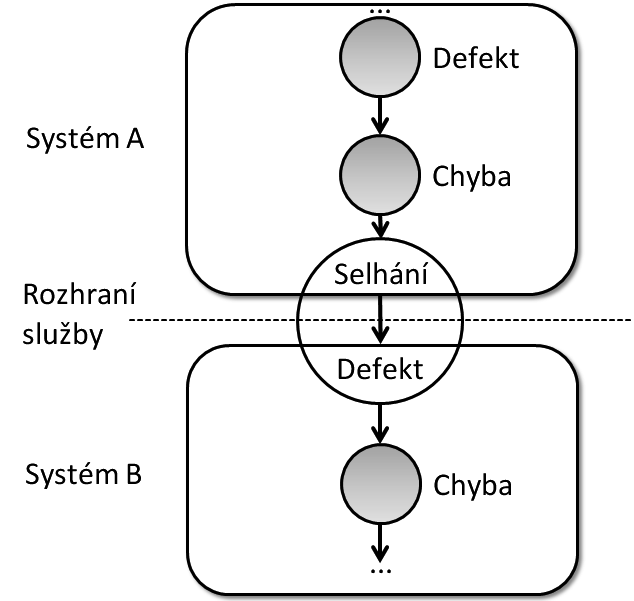
\includegraphics[width=8cm]{img/Bug.png}
	\end{figure}
	
	\section{Testování softwaru}
	Definice pojmu testování softwaru se více či méně liší téměř v~každé publikaci. V~knize \citep{RizeniKvalitySW} je testování definováno jako proces řízeného spouštění softwarového produktu s cílem zjistit, zda splňuje specifikované či implicitní potřeby uživatelů. Je zde důležité slovo spouštění, které z~testování vyřazuje metody statické analýzy. Obecněji se však i~tyto metody do testovaní řadí a~jejich použití bývá ve vývoji softwaru vhodné.
	
	Záměrem testování již není nalézat defekty, jak tomu bylo dříve. Nyní je jím získat informaci o~kvalitě softwaru a~o~tom, jak moc splňuje požadavky zákazníka.
	
	\citep{Patton} uvádí řadu axiomů (obecně přijímaných pravd, které se nemusejí dokazovat) o~testování. Čtyři nejdůležitější z~nich jsou:
		\begin{itemize}
			\item Žádný program není možné otestovat kompletně -- počet vstupů, výstupů a cest, které vedou skrze software je příliš velký.
			\item Testování softwaru je postavené na riziku -- nemožnost otestování všech případů vede k~tomu, že je možné nezachytit defekt ve scénáři, který se netestoval. Je proto důležité správně odhadnout možná rizika a~testováním je minimalizovat.
			\item Testování nikdy nemůže prokázat, že chyby neexistují -- testováním pouze můžeme dokázat, že chyby existují, ale jelikož není možné software kompletně otestovat, existenci chyb vyloučit nelze.
			\item Čím více chyb najdeme, tím více jich v~softwaru je -- kvůli tomu, že programátoři mívají špatné dny nebo dělají často stejné chyby, se chyby vyskytují ve skupinách. To znamená, že objevení jedné chyby zvyšuje pravděpodobnost dalších takových podobných chyb.
		\end{itemize}
		
		\section{Úrovně testování}
		Během vývoje softwaru se testování nechá rozdělit do různých skupin, např. podle toho, kdy se testování provádí, jakým způsobem se provádí, jak se k~testované aplikaci přistupuje, či jaká část aplikace se podrobuje testům. Rozlišují se např. tyto čtyři fáze:
			\begin{itemize}
				\item Testování jednotek (Unit Testing) -- testování provádí obvykle sám programátor, který se snaží prokázat správnost fungování jednotlivých jednotek (nejmenších testovatelných součástí aplikace).
				\item Integrační testování (Integration Testing) -- testuje se zapojení výše uvedených jednotek do aplikace. Správná funkčnost jednotek nezaručuje správnou funkčnost výsledné aplikace.
				\item Systémové testování (System Testing) -- testuje se, zda aplikace splňuje požadavky zákazníka. Patří sem nejen funkční testování, ale i~mimofunkční.
				\item Akceptační testování (User Acceptance Testing, UAT) -- zde provádí testování sám zákazník a~neomezuje se pouze na testování jako takové, ale na splnění před dohodnutých kritérii (dokumentace, manuály apod.).
			\end{itemize}
			
		\section{Testování uživatelského rozhraní}
		Podle \citep{Patton} má každá aplikace uživatelské rozhraní (UI - user interface). V~dnešní době je dělíme do dvou skupin, grafické (GUI - graphical user interface) a~z~příkazové řádky (CLI - command line interface). V~obou případech UI slouží pro interakci a~komunikaci s~uživatelem. Je to prostředek pro zadavání vstupních data a~získávání výstupů.
		
		Použitelnost UI znamená, nakolik funkční a~efektivní je práce uživatele s~programem. K~tomu se vztahuje pojem ergonomika -- zabývá se návrhem a~konstrukcí předmětů s~ohledem na to, aby se s~nimi pracovalo jednoduše. Vzhledem k~použitelnosti se tedy bude testovat, zda je aplikace těžko srozumitelná, obtížně se s~ní pracuje, je pomalá, nebo ji zákazník nebude považovat za vyhovující.
		
		Dobré uživatelské rozhraní by mělo mít následující vlastnosti:
			\begin{itemize}
				\item Dodržuje standardy nebo zásady -- pokud aplikace poběží na specifické platformě, je možné, že pro tuto platformu existují předepsané standardy a~normy na vzhled a~chování aplikací (tzv. look and feel), které je vhodné dodržovat.
				\item Je intuitivní -- míry intuitivnosti softwaru jsou např.: Je UI zřetelné, vhodně rozložené? Nepřekáží vám v tom, co s ním hodláte dělat? Nachází se funkce a~odpovědi tam, kde je očekáváte? Je jasné, co bude další akce v~pořadí? Není příliš komplikované (neobsahuje moc funkcí)?
				\item Je konzistentní -- uživatelé si zvyknou na určitý způsob ovládání a~očekávají, že provedou stejnou akci velmi podobně i~v~jiném programu. Proto je důležité věnovat pozornost nejen konzistenci v~rámci naší aplikace, ale i~vůči ostatním. Pozor bychom si měli dávat na klávesové zkratky, výběry z~nabídek, umístění tlačítek, výstupy aplikace apod.
				\item Je flexibilní -- uživatelé mají rádi možnost volby. I~v~jednoduchých programech typu kalkulačka bývá na výběr alespoň ze dvou rozložení -- standardního a~věděckého. To ovšem znesnadňuje testování, proto by voleb nemělo být příliš mnoho.
				\item Je pohodlné -- software by neměl uživateli práci s~ním nijak znepříjemňovat. Je vhodné zaměřit se na náležitost (měl by působit dojmem, který odpovídá jeho záměru), ošetření chyb (upozornění před kritickou operací, návrat o~krok zpět aj.), rychlost zpracování (chybové hlášky zobrazovat dostatečně dlouho, uvést odhadovaný čas do dokončení).
				\item Je správné -- ověřuje se to, zda UI dělá to, co má. Pozornost by se měla věnovat marketingovým rozdílům (v~aplikaci nejsou oproti marketingovým dokumentům funkce navíc, nebo chybějící funkce), jazyku a~pravopisu, nesprávným médiím (různorodé ikony, zvuky a~jiné části UI).
				\item Je užitečné -- přispívají dané funkce zvýšení užitné hodnoty aplikace? Pomůže uživateli v~jeho práci s~aplikací? Nepodstatné funkce znamenají zbytečné testování navíc a~pro zákazníka mohou být špatné.
			\end{itemize}
		
		\section{Automatizace testování}
		Důvodem automatizace testování je zvýšení jeho efektivity. Manuální návrh, provedení a~analýza testů je časově náročná a~často velice monotónní práce. Testeři mohou jednak ušetřit čas, a~jednak se sníží pravděpodobnost chybného vykonání testu z~důvodu ztráty koncentrace testera v~důsledku jednotvárné činnosti. Dalším přínosem je průběžně se stále zvětšující sada regresních testů. Ty slouží k~otestování, zda nově přidaná funkcionalita či úprava aplikace nezpůsobuje chyby v~již funkčních částech.
		
		Funkcionální testování UI je jednou z~částí testování UI, která se nechá automatizovat. Existuje celá řada nástrojů, které umožňují simulování klikání a~psaní na klávesnici. Další částí vhodnou pro automatizaci je kontrola, zda GUI obsahuje všechny prvky, a~jestli je chování prvků konzistentní a~stejné, jako požadované. V~obou těchto disciplínách je pro nástroj důležité, aby zvládal klikat a~psát do aplikace, ale zároveň vyhodnocoval její stav (vstup je možné zadávat až tehdy, když je na to aplikace připravená, apod.).
		
			\subsection{Monkey testování}\label{MonkeyTestovani}
			Specifickou oblastí testování GUI a~automatického testování je tzv. monkey testování (testování za pomoci \emph{cvičené opice}). To vychází z~\uv{Nekonečného opičího teorému}, \citep{Patton}, \citep{Teorem}, který říká: \uv{Pokud by měli po nekonečnou dobu k~dispozici nekonečně mnoho opic, které by neustále náhodně psaly na nekonečně mnoho klávesnic, statisticky vzato by mohly nakonec napsat všechny Shakespearovy hry.}
			
			Nejde o~automatizaci za účelem usnadnění práce a~zvýšení efektivity, ale za účelem napodobit možné chování potenciálního uživatele. Přes všechno naše snažení a~testování určitě v~aplikaci zůstaly chyby, které by odhalil případný uživatel podobným nezasvěceným klikáním a~psaním. Tomu je však možné alespoň částečně předejít pomocí monkey testování.